\documentclass{report}
\usepackage[UTF8]{ctex}
\usepackage{amsmath}
\usepackage{algorithm}
\usepackage{algorithmicx}
\usepackage[noend]{algpseudocode}
\usepackage{bm}
\usepackage{booktabs}
\usepackage{cite}
\usepackage[top=1in,bottom=1in,left=1.25in,right=1.25in]{geometry}
\usepackage[colorlinks,linkcolor=blue]{hyperref}
\usepackage{graphicx}
\usepackage{hyperref}
\usepackage{listings}
\usepackage{longtable}
\usepackage{tikz}
\usepackage{xcolor}
\graphicspath{{figures/}}

\lstset{
  basicstyle=\footnotesize,       % the size of the fonts that are used for the code
  numbers=left,                   % where to put the line-numbers
  numberstyle=\tiny\color{gray},  % the style that is used for the line-numbers
  stepnumber=1,                   % the step between two line-numbers. If it's 1, each line will be numbered
  numbersep=5pt,                  % how far the line-numbers are from the code
  backgroundcolor=\color{white},  % choose the background color. You must add \usepackage{color}
  showspaces=false,               % show spaces adding particular underscores
  showstringspaces=false,         % underline spaces within strings
  showtabs=false,                 % show tabs within strings adding particular underscores
  frame=single,                   % adds a frame around the code
  rulecolor=\color{black},        % if not set, the frame-color may be changed on line-breaks within not-black text (e.g. commens (green here))
  tabsize=2,                      % sets default tabsize to 2 spaces
  captionpos=b,                   % sets the caption-position to bottom
  breaklines=true,                % sets automatic line breaking
  breakatwhitespace=false,        % sets if automatic breaks should only happen at whitespace
  keywordstyle=\color{blue},      % keyword style
  commentstyle=\color{dkgreen},   % comment style
  stringstyle=\color{red},        % string literal style
}

\title{图像实验结题报告}
\author{无76 \hspace{2ex} RainEggplant \hspace{2ex} 2017****** \\
无76 \hspace{2ex} AAA \hspace{2ex} 2017****** \\
无76 \hspace{2ex} BBB \hspace{2ex} 2017******}

\begin{document}
\maketitle
\tableofcontents
\newpage

\chapter{简介}

本次大作业我们聚焦于交通标志的分类、单样本分类与检测问题。
基于几种成熟模型或框架,我们完成了相应的编程和调优工作。
具体地,RainEggplant 同学负责任务一和任务二;AAA 同学负责任务三;BBB 同学负责任务四。
本结题报告将以四个任务为顺序展开,分别包括各部分的文献调研、方法原理、方案设计、实验结果、问题与反思等。

\chapter{文献调研}

\section{交通标志分类} \label{sec:classification}
通常来说,交通标志有着独特和易于区分的特征。例如,其形状简单,一般为三角形或圆形;其用色较统一,图案对比度较高。因此,交通标志的检测和分类是一个约束性的问题。但尽管如此,设计一个精准、可靠而高效的交通标志识别系统仍然颇具挑战性。在实际场景中,由于环境复杂多变和设备限制等因素,系统获取的交通标志的图像通常存在尺寸不一、视角不同、模糊发虚、色彩暗淡、物体遮挡以及光照情况不同等问题 \cite{STN-CNN}。

交通标志分类的研究方法按时间顺序分为几个阶段。最初阶段的方法通常基于颜色或形状,其非常依赖于研究者自主设计的算法和特征选取方法 \cite{STN-CNN}。第二阶段的方法由传统的机器学习方法主导。这些方法主要基于 HOG (Histogram of Oriented Gradients)、 SURF (Speeded Up Robust Features)、SIFT (Scale Invariant Feature Transform)、RIBP (Rotation Invariant Binary Pattern)、LBP (Local Binary Pattern) 等特征,采用 SVM、随机森林、最近邻等算法进行分类 \cite{STN-CNN,MTCNN,HOG-SURF}。然而,该类方法普遍存在的需要手动提取特征,而设计一个好的特征是非常困难而耗费精力的 \cite{MTCNN}。近年来,深度学习的迅速发展推动交通标志分类进入了第三个阶段。这一阶段最具代表性的方法是基于 CNN (Convolutional Neural Networks) 的分类方法。CNN 能够自动提取高级的特征,具有很强的适应能力,非常适合用于交通标志的分类。此外,还出现了结合手工特征与 CNN \cite{HOG-SURF}、引入 STN (Spatial Transformer Networks) 到 CNN \cite{STN-CNN} 等多种变体。以下将结合调研的文献,介绍部分交通标志分类算法。

\subsection{基于传统机器学习的分类}

基于传统机器学习的分类方法需要手工特征作为输入以训练分类器。此处介绍一种分类准确度较高的算法。

Mathias 等人于 2013 年提出的细粒度分类算法 \cite{Mathias} 在 GTSRB \cite{GTSRB} 上取得了 98.53\% 的识别准确率,在基于传统机器学习的分类中位居第一。其工作流程分为三步:特征提取、降维和分类。其合并了交通标志图像的灰度值以及基于 HOG 的特征,采用 INNLP (Iterative Nearest Neighbours-based Linear Projections) 方法降维,最后使用 INNC (Iterative Nearest Neighbours) 方法进行分类。

\subsection{基于深度学习的分类}

\subsubsection{预处理}

基于深度学习的分类算法通常直接采用图像作为输入,不需要手工提取特征。但是,正如 \ref{sec:classification} 节所提到的,用于训练的图像存在多方面的差异。此外,不同类别的训练样本个数也不一定相等。因此需要对数据进行预处理。

常见的预处理方法包括但不限于:

\begin{itemize}
  \item 标准化
  \item 图像处理:例如更改尺寸、直方图均衡化、边缘增强等方法
  \item 数据扩充:由原数据生成经旋转、镜像等操作后的数据
\end{itemize}

视算法具体情况,通常会采用一种或多种预处理方法,最终获得尺寸一致、各类样本数接近的训练样本。

\subsubsection{改进型方法范例}

尽管普通的 CNN 分类方法有不错的成绩,但其在很多方面仍有改进的空间,例如复杂度、准确性等。许多研究者就此提出改进后的方法或其他变体,取得了明显的效果。下面介绍一些改进型方法。

CireşAn \cite{MCDNN} 等人在 2012 年提出了多列深度神经网络 (MCDNN)。其思想是对训练集采用不同的预处理操作得到多个样本集合,再分别用这些样本去训练各个 DNN,分类结果是各个 DNN 结果的平均。在这一工作中,CireşAn 采用 5 种预处理训练了 25 个 DNN,在 GTSRB 上取得了 99.46\% 的识别准确率。

Madan \cite{HOG-SURF} 等人于 2019 年提出了基于 HOG-SURF 混合特征的分类方法,旨在利用手工特征降低模型复杂度。HOG 特征倾向于提取到全局信息且对光照不敏感,但其对于物体分方位敏感;而 SURF 特征具有旋转不变性。两类特征可以互补。这一工作在 GTSRB 上取得了 98.48\% 的识别准确率。

Arcos-García \cite{STN-CNN} 等人将 STN 引入了 CNN, 抛弃了对数据进行扩充以及采用多个并行的 CNN 的做法。STN 可以学习到几何变换的参数,从而使得网络对于输入图像的几何变形有很强的适应力。该工作在 GTSRB 上取得了 99.71\% 的识别准确率,是目前准确率最高的分类算法。

\subsection{单样本分类问题}

\emph{略。}

\section{交通标志检测}

\emph{略。}

\chapter{基于传统机器学习的分类}

\section{方法原理}

经过文献调研,我们最终选择了文献 \cite{Mathias} 提出的细粒度分类方法作为主要的参考思路。我们提出的方法包含三个阶段:特征提取、特征降维和分类。下面将详细介绍每一阶段的基本原理。

\subsection{特征提取}

由于交通标志的设计考虑到了色盲人群,其最突出的区分性特征是它的内部图案和形状,而色彩相对而言并不重要。文献 \cite{Mathias} 尝试使用了色彩相关的特征,但其分类效果不如只使用灰度相关的特征的方法,并且使用了色彩相关的特征还会增加计算复杂度。因此,我们丢弃了图像的彩色信息。

在实验中,我们使用了如下特征:

\paragraph{I}
缩放为 $28 \times 28$ 大小的图像的灰度值。I 特征具有 784 维。

\paragraph{PHOG}
即 HOG 金字塔特征 (pyramid of histograms of oriented gradients)。我们采用了文献 \cite{Digit} 中的实验所使用的最佳参数。PHOG 特征具有 2172 维。

\paragraph{HOG1, HOG2, HOG3}
我们采用了文献 \cite{GTSRB} 中的参数设置,计算了三类 HOG 特征,它们具有不同的 cell 大小和采样格点。HOG1, HOG2 特征都具有 1568 维,HOG3 特征具有 2916 维。

\subsection{特征降维}

我们使用线性判别分析 (LDA) 进行特征降维。其思想是向低维度投影后,类内方差最小而类间方差最大。其结果可以通过求解特征值问题求得。因为我们的样本共有 19 类,因此经过 LDA 降维后,特征变为 18 维。需要注意的是,为了改善样本与特征维数之比较小时的结果,我们使用了正则化的 LDA。

\subsection{分类}

我们使用 SVM,构造了 One-vs-Rest 分类器进行分类,核函数选用径向高斯核 (RBF)。

\section{方案设计}

我们采用 python 上的 sklearn 库实现了上述分类方法。我们从零编写代码,实现了 PHOG 和 HOGx 特征的提取,其函数位于 hog\_x.py 和 phog.py 中,我们将其封装在 feature\_extractor.py 中,作为特征提取器。详情情参考代码。

对外部,我们提供了三个调用接口。

\begin{itemize}
  \item extract.py: 接受训练集、测试集的路径为输入,提取其特征保存到输出文件。
  \item train.py: 接受训练集、训练集特征的路径为输入,训练后保存模型到输出文件。此外,还可以划分验证集对训练效果进行评估。
  \item predict.py: 接受测试集、测试集特征的路径和模型文件为输入,输出预测结果。
\end{itemize}

\section{实验结果}

我们选取了 70\% 的样本作为训练集,余下为测试集。我们的方法在训练集上的准确率为 99.7\%, 测试集上的准确率为 97.0\% .

\section{问题与反思}

我们可以从方法的三个阶段切入,思考现阶段存在的问题和进一步的改进思路。在特征选取上,目前的选取的几类特征都基于 HOG 特征,可能存在一定的冗余。同时,因为特征维数较大,在进行 LDA 降维时复杂度较高。另一方面,在前期调研中,我们还注意到有使用 HOG + SURF 混合特征的方法 \cite{HOG-SURF},这提示我们可以尝试加入其他类型的特征。在特征降维上,文献 \cite{Mathias} 还提到了 SRLP (Sparse Representation based Linear Projection) 和 INNLP (Iterative Nearest Neighbours-based Linear Projections) 方法,其中 INNLP 在文献的问题中取得了最好的效果,因此二者也是可以尝试的降维方法。在分类上,还可以与最近邻分类、SRC (Sparse Representation-based Classifier)、INNC (Iterative Nearest Neighbors Classifier) 等分类方法的分类效果进行对比,选出最优的分类方法。

\chapter{基于深度学习的分类}

\section{方法原理}

经过文献调研,我们发现在基于深度学习的分类方法中,文献 \cite{STN-CNN} 提出的基于引入 STN (Spatial Transformer Network) 的 CNN 的分类方法在 GTSRB 数据集 \cite{GTSRB} 具有最高的识别准确率(99.71\%)。因此,我们采用了该文献的网络结构。

\subsection{数据预处理}

在数据预处理阶段,我们将所有图片缩放到 $48 \times 48$ 尺寸,并执行了全局的 Normalization。

\subsection{STN}

空间变换网络 (STN) \cite{STN} 能够对输入进行几何变换,从而能够以高效的方式使得 CNN 对输入具有空间不变性。从而,我们可以省去额外的训练监督、手工的数据增强(例如旋转、平移、放缩、扭曲、翻转)或者数据的归一化技巧 \cite{STN-CNN}。

\begin{figure}[htbp]
  \centering
  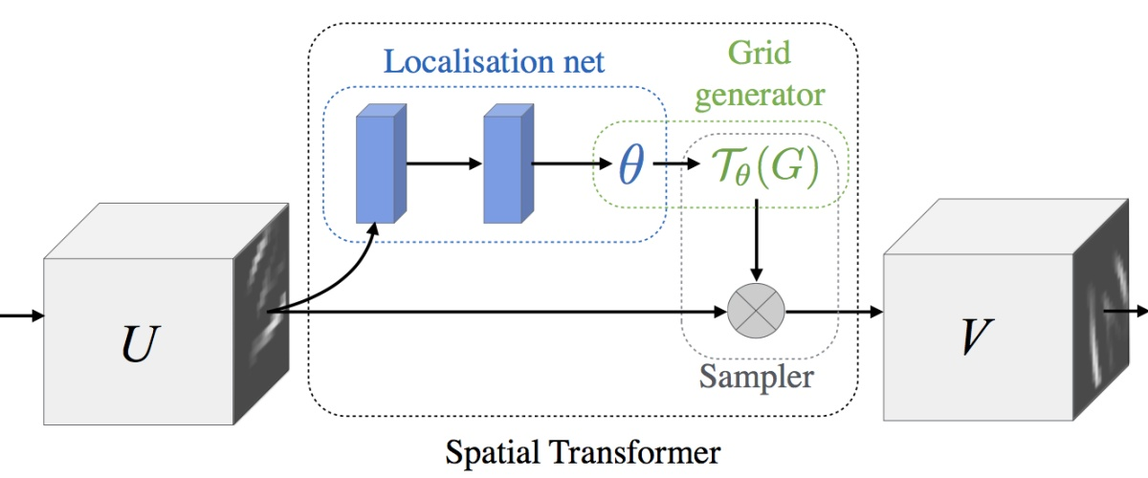
\includegraphics[width = 0.6 \textwidth]{STN.png}
  \caption{STN 的构成 \cite{STN}}
  \label{fig:STN}
\end{figure}

STN 由三部分组成:localisation net, grid generator 和 sampler (见图 \ref{fig:STN})。Localisation net 是一个普通的 CNN, 其作用是学习变换矩阵的参数 $\theta$。Grid generator 输出特征图的坐标点对应输入特征图的坐标点的位置。其计算方式如式 \ref{eq:affine-transform} 。Sampler 则是利用给定的插值方式计算对应点的值。

\begin{equation}
\begin{pmatrix}
x_i^s \\ y_i^s
\end{pmatrix} =
A_\theta
\begin{pmatrix}
x_i^t \\ y_i^t \\ 1
\end{pmatrix} =
\begin{bmatrix}
\theta_{11} & \theta_{12} & \theta_{13} \\
\theta_{21} & \theta_{22} & \theta_{23}
\end{bmatrix}
\begin{pmatrix}
x_i^t \\ y_i^t \\ 1
\end{pmatrix}
\label{eq:affine-transform}
\end{equation}

STN 可以很方便地插入到 CNN 的结构里。在本实验中,STN 能够去除输入图片中不相关的几何噪声和背景,校正尺寸和方向,截取感兴趣的部分传递到下一层网络 \cite{STN-CNN}。

\subsection{Local Contrast Normalization}

LCN 能够通过 subtractive local normalisation 和 divisive local normalisation 对图像执行局部对比度归一化。在这里我们使用的是高斯核。

\section{方案设计}

\subsection{网络结构}

\begin{figure}[htbp]
  \centering
  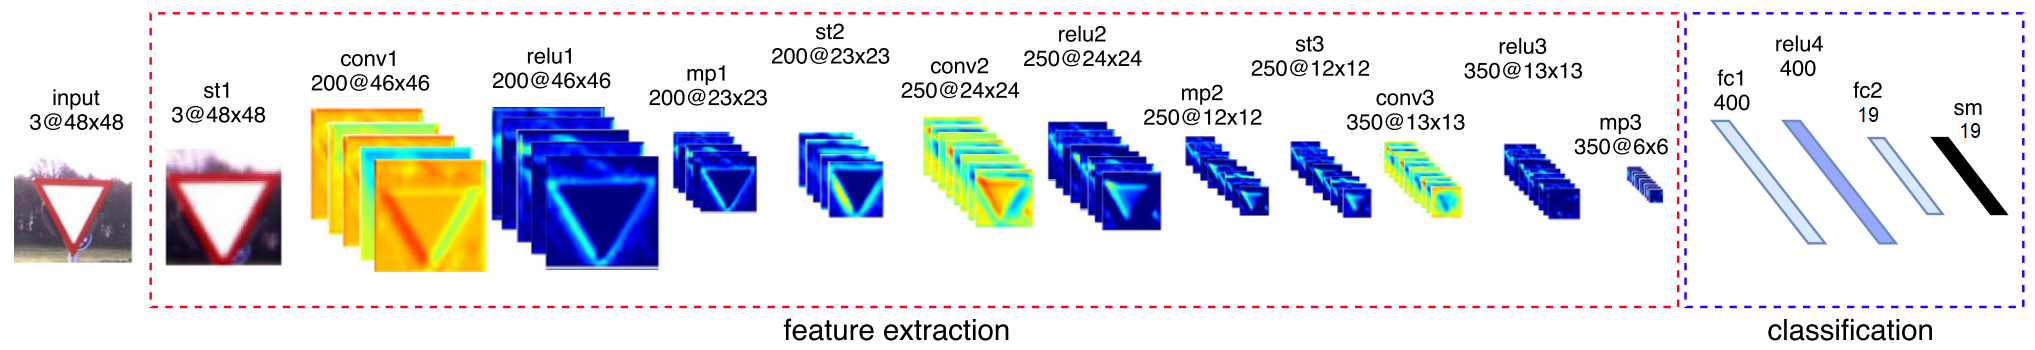
\includegraphics[width = 1 \textwidth]{STN-CNN.png}
  \caption{网络结构}
  \label{fig:network}
\end{figure}

我们的网络结构如 \ref{fig:network} 所示。注意图中省略了 LCN 和 STN 的 localisation net。

表 \ref{tbl:network} 详细展示了具体的网络参数。

\begin{longtable}[]{@{}llll@{}}
  \caption{\label{tbl:network}网络结构}\tabularnewline
  \toprule
  层 & 类型 & \# Maps \& neurons & Kernel\tabularnewline
  \midrule
  \endfirsthead
  \toprule
  层 & 类型 & \# Maps \& neurons & Kernel\tabularnewline
  \midrule
  \endhead
  0 & Input & 3 m. of 48 × 48 n. &\tabularnewline
  1 & STN1 & &\tabularnewline
  2 & Convolutional & 200 m. of 46 × 46 n. & 7 × 7\tabularnewline
  3 & ReLU & 200 m. of 46 × 46 n. &\tabularnewline
  4 & Max-Pooling & 200 m. of 23 × 23 n. & 2 × 2\tabularnewline
  5 & Local Contrast Norm. & 200 m. of 23 × 23 n. &\tabularnewline
  6 & STN2 & &\tabularnewline
  7 & Convolutional & 250 m. of 24 × 24 n. & 4 × 4\tabularnewline
  8 & ReLU & 250 m. of 24 × 24 n. &\tabularnewline
  9 & Max-Pooling & 250 m. of 12 × 12 n. & 2 × 2\tabularnewline
  10 & Local Contrast Norm. & 250 m. of 12 × 12 n. &\tabularnewline
  11 & STN3 & &\tabularnewline
  12 & Convolutional & 350 m. of 13 × 13 n. & 4 × 4\tabularnewline
  13 & ReLU & 350 m. of 13 × 13 n. &\tabularnewline
  14 & Max-Pooling & 350 m. of 6 × 6 n. & 2 × 2\tabularnewline
  15 & Local Contrast Norm. & 350 m. of 6 × 6 n. &\tabularnewline
  16 & Fully connected & 400 neurons & 1 × 1\tabularnewline
  17 & ReLU & 400 neurons &\tabularnewline
  18 & Fully connected & 19 neurons & 1 × 1\tabularnewline
  19 & Local Contrast Norm. & 19 neurons &\tabularnewline
  \bottomrule
\end{longtable}

其中,三个 STN 的 localisation net 的结构如 表 \ref{tbl:stn} 所示。

\begin{longtable}[]{@{}llll@{}}
  \caption{\label{tbl:stn}STN 的 localisation net 的结构}\tabularnewline
  \toprule
  层/类型 & Loc. net of ST 1 & Loc. net of ST 2 & Loc. net of ST3\tabularnewline
  \midrule
  \endfirsthead
  \toprule
  层/类型 & Loc. net of ST 1 & Loc. net of ST 2 & Loc. net of ST3\tabularnewline
  \midrule
  \endhead
  0/Input & 3 of 48 × 48 & 200 of 23 × 23 & 250 of 12 × 12\tabularnewline
  1/Max-Pool & 3 of 24 × 24 & 200 of 11 × 11 & 250 of 6 × 6\tabularnewline
  2/Conv & 250 of 24 × 24 & 150 of 11 × 11 & 150 of 6 × 6\tabularnewline
  3/ReLU & 250 of 24 × 24 & 150 of 11 × 11 & 150 of 6 × 6\tabularnewline
  4/Max-Pool & 250 of 12 × 12 & 150 of 5 × 5 & 150 of 3 × 3\tabularnewline
  5/Conv & 250 of 12 × 12 & 200 of 5 × 5 & 200 of 3 × 3\tabularnewline
  6/ReLU & 250 of 12 × 12 & 200 of 5 × 5 & 200 of 3 × 3\tabularnewline
  7/Max-Pool & 250 of 6 × 6 & 200 of 2 × 2 & 200 of 1 × 1\tabularnewline
  8/Fc & 250 neurons & 300 neurons & 300 neurons\tabularnewline
  9/ReLU & 250 neurons & 300 neurons & 300 neurons\tabularnewline
  10/Fc & 6 neurons & 6 neurons & 6 neurons\tabularnewline
  \bottomrule
\end{longtable}

\subsection{代码实现}

我们采用 python 上的 PyTorch 实现了该神经网络。其中,我们手动实现了 local contrast normalizer 网络和 spatial transformer 网络的定义,分别封装在 modules 文件夹下的 local\_contrast\_normalizer.py 和 spatial\_transformer.py 中。我们的网络模型定义在 stn\_cnn.py 中。我们采用了 PyTorch-Lightning 库来简化工程代码、跟踪训练情况。

对外部,我们提供了两个调用接口。

\begin{itemize}
  \item train.py: 接受训练集的路径、训练器参数、保存点等为输入,输出训练评价指标、保存点。
  \item predict.py: 接受保存点、测试集为输入,输出预测结果。
\end{itemize}

\section{实验结果}

STN 能自动学习几何变换的参数,对输入的图像进行变换。如图 \ref{fig:stn_process} 所示,左侧为输入 STN 前的图像,右图为 STN 输出的图像。可以看到,STN 网络对输入图像进行了裁剪、旋转、扭曲等仿射变换。这使得我们的 CNN 网络具有了一定的空间不变性。

\begin{figure}[htbp]
  \centering
  
\includegraphics[width = 0.2 \textwidth]{stn-process.png}
  \caption{图像经过 STN 处理前后}
  \label{fig:stn_process}
\end{figure}

我们采用普通的 SGD 优化算法,设定学习率为 0.01,batch size 为 50,使用交叉熵损失函数。按 8:2 的比例划分训练集和测试集,在 16 epochs 时, 网络在测试集上的准确率达到了 98.76\%。图 \ref{fig:cnn-loss} 展示了训练过程中的训练集损失曲线,图 \ref{fig:cnn-accuracy} 展示了验证集准确率曲线。

\begin{figure}[htbp]
  \centering
  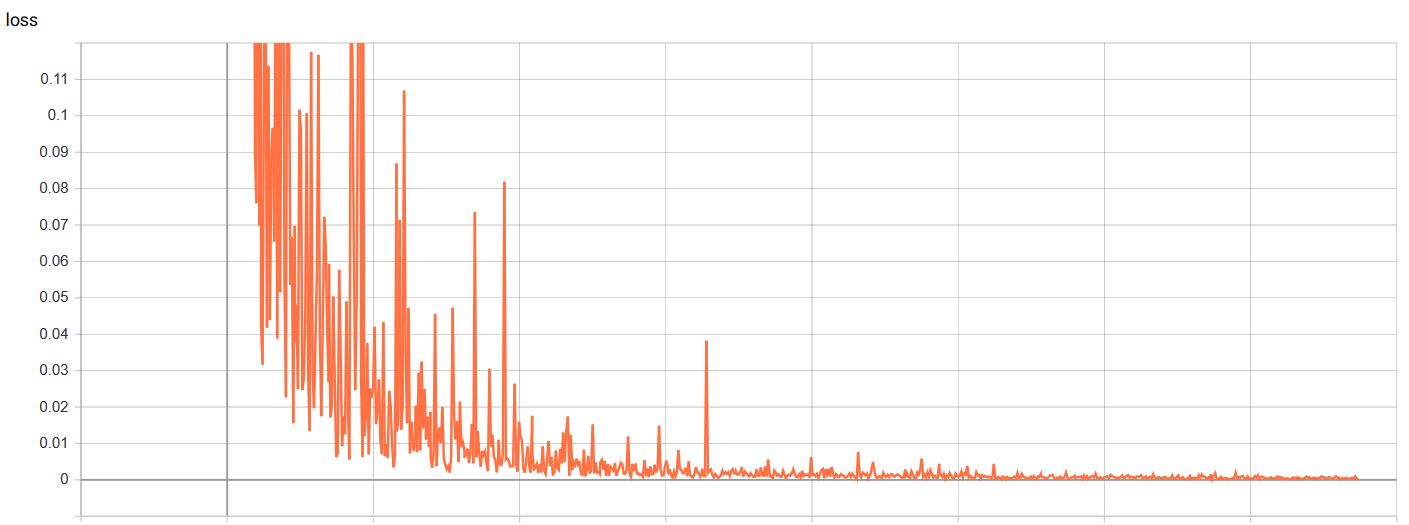
\includegraphics[width = 0.9 \textwidth]{cnn-loss.jpg}
  \caption{训练集损失曲线}
  \label{fig:cnn-loss}
\end{figure}

\begin{figure}[htbp]
  \centering
  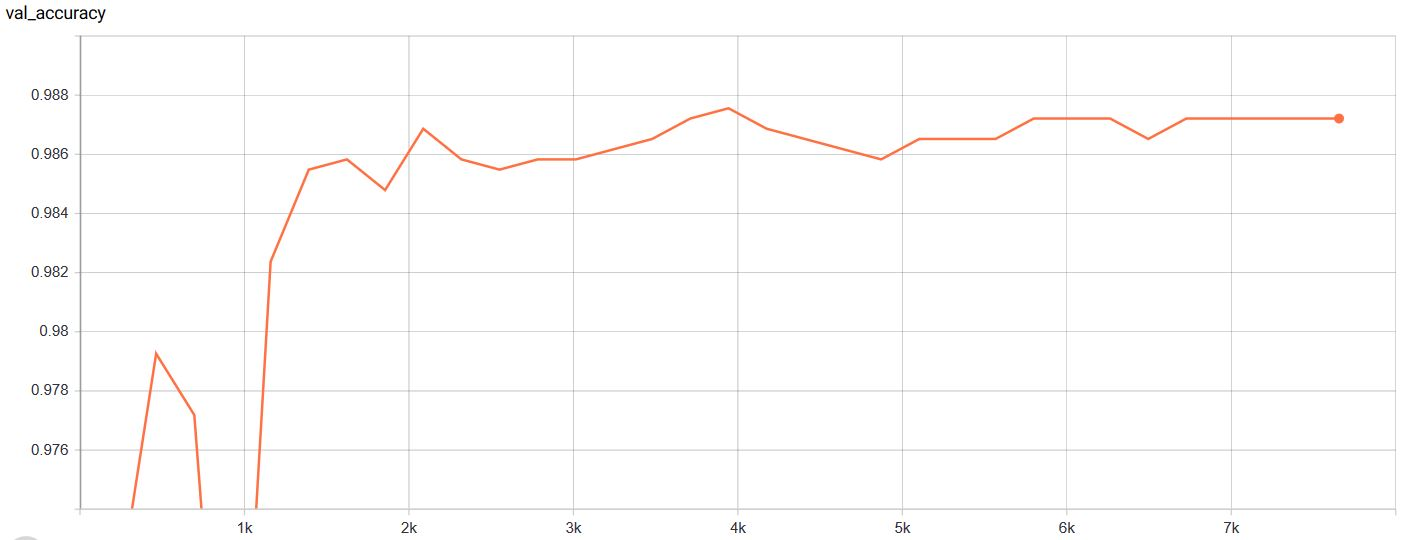
\includegraphics[width = 0.9 \textwidth]{cnn-val-accuracy.JPG}
  \caption{验证集准确率曲线}
  \label{fig:cnn-accuracy}
\end{figure}


\section{问题与反思}

在 CNN 中引入 STN 是一次很有意义的尝试,事实证明,通过引入 STN,我们赋予了 CNN 较强的空间不变性,省去了一系列无趣而麻烦的数据增强操作。

然而我们的项目也存在着问题。我们完全采用了文献 \cite{STN-CNN} 所提出的网络结构。但是,其使用的数据集是 GTSRB,这是一个比我们的实验数据集更大的数据集,有 43 类标志牌,训练集有 39209 张图片。因此,这样的网络结构对于我们的课题可能过大了,而这除了会增加计算量,还可能导致过拟合现象。因此,有针对性地调整网络参数应当会进一步提升准确率和减少计算量。此外,我们仅使用了 SGD 作为优化方法,并未尝试其他优化方法在本课题上的表现。

\chapter{单样本分类问题}

\emph{略。}

\chapter{交通标志检测}

\emph{略。}

\bibliographystyle{IEEEtran}
\bibliography{ref}
\end{document}
